% =========================================================
%  Chapter 5 — Semiconductor Light Sources: Fundamentals and Review
%  Source: Dr. George's Lectures (Lecture 1)
%  Style: student-voice notes matching the personal style guide
% =========================================================

% ------------------------------------------------------------------
\section{Why Semiconductors?}
% ------------------------------------------------------------------

To understand how a laser diode works, we must first understand the material it is built from. Semiconductors sit in a peculiar middle ground — they are not metals (which conduct electrons freely) and not insulators (which block them entirely). The interesting physics happens precisely in that gap: a \textbf{bandgap} separating a filled valence band from an empty conduction band. By injecting extra carriers into a semiconductor — or by forward-biasing a PN junction — we can create conditions where photons are \emph{emitted} rather than absorbed. That is the entire engine behind the LED and the laser diode, and why this review is essential.

Before we write down a single carrier concentration formula, we need to build the physical picture from the ground up: what does the energy structure of a semiconductor actually look like, and what determines how many electrons or holes live at any given energy?

% ------------------------------------------------------------------
\section{The Energy Band Structure}
% ------------------------------------------------------------------

\subsection{From Discrete Levels to Continuous Bands}

In an isolated atom, electrons occupy perfectly sharp, discrete energy levels. When billions of atoms are packed into a crystal lattice, those levels broaden into continuous \textbf{energy bands} because the electrons now interact with every neighbouring ion simultaneously. Two bands are particularly important for optoelectronics:

\begin{itemize}
    \item \textbf{Valence Band (VB):} The highest energy band that is essentially \emph{full} of electrons at absolute zero. Electrons here are bound to atoms and do not contribute to conduction.
    \item \textbf{Conduction Band (CB):} The next band above the valence band, which is essentially \emph{empty} at absolute zero. Electrons promoted into this band are free to move and carry current.
\end{itemize}

Between these two bands sits the \textbf{bandgap} $E_g$, defined as:
\begin{equation*}
    E_g = E_c - E_v
\end{equation*}
where $E_c$ is the energy of the conduction band edge (the \emph{minimum} energy an electron in the CB can have) and $E_v$ is the energy of the valence band edge (the \emph{maximum} energy an electron in the VB can have). No electron state exists anywhere inside this forbidden gap.

The physical takeaway here is that a photon can only be absorbed if its energy exceeds the bandgap: $h\nu > E_g$. Conversely, when an electron falls from the CB back into the VB, it releases approximately $E_g$ worth of energy — ideally as a photon.

\subsection{The E–k Diagram and Effective Mass}

The most compact and powerful way to describe the band structure of a semiconductor is the \textbf{dispersion relation} $E(k)$ — a plot of electron energy $E$ against crystal momentum $\hbar k$. This is called the \textbf{E–k diagram}.

Near the band edges, where the interesting physics happens, the bands are approximately parabolic. The curvature of this parabola encodes how easily the electron accelerates in response to an applied force. We define the \textbf{effective mass} $m^*$ precisely through this curvature:
\begin{keyresult}
\begin{equation}
    \frac{1}{m^*} \equiv \frac{1}{\hbar^2}\,\frac{d^2 E}{dk^2}
\end{equation}
\end{keyresult}
where $\hbar$ is the reduced Planck constant and $k$ is the wavenumber. A large curvature (sharply peaked band) means a small effective mass — the electron responds strongly to applied forces and behaves as if it were light. A flat band gives a large effective mass — the electron is sluggish. This substitution of the free electron mass $m_0$ with the material-specific effective mass $m^*_e$ (for electrons in the CB) or $m^*_h$ (for holes in the VB) lets us treat carriers as free particles obeying familiar Newtonian dynamics, but with mass $m^*$ instead of $m_0$.

Near the conduction band minimum $E_c$, the parabolic approximation gives:
\begin{equation*}
    E(k) \approx E_c + \frac{\hbar^2 k^2}{2 m^*_e}
\end{equation*}
and near the valence band maximum $E_v$ for holes:
\begin{equation*}
    E(k) \approx E_v - \frac{\hbar^2 k^2}{2 m^*_h}
\end{equation*}

The negative sign for holes follows from the fact that removing an electron from the valence band leaves a hole whose energy \emph{increases} as it moves deeper into the band (i.e., further away from $E_v$).

% ------------------------------------------------------------------
\section{Direct and Indirect Bandgaps}
% ------------------------------------------------------------------

Not all semiconductors are equal for optoelectronic applications. The most critical distinction is whether the semiconductor has a \textbf{direct} or \textbf{indirect} bandgap.

An optical transition requires \emph{both} conservation of energy and conservation of momentum. The photon satisfies energy conservation:
\begin{equation*}
    E_2 - E_1 = E_\text{ph} = h\nu
\end{equation*}
But momentum conservation places a severe additional constraint. The photon carries momentum $p_\text{ph} = \hbar k_\text{ph}$, and the change in electron momentum must equal it:
\begin{equation*}
    \hbar(k_2 - k_1) = \hbar k_\text{ph}
\end{equation*}
Now, the electron wavevector in the crystal is of order $k_\text{electron} \sim 2\pi/a \sim 10^{10}\ \text{m}^{-1}$, where $a$ is the lattice constant ($\sim 5\,\text{\AA}$). The photon wavevector, by contrast, is $k_\text{ph} = 2\pi/\lambda \sim 10^{6}\ \text{m}^{-1}$ for visible/near-IR light. Since $10^6 \ll 10^{10}$, the photon carries essentially no momentum on the scale of the Brillouin zone. Therefore, momentum conservation demands:
\begin{keyresult}
\begin{equation}
    k_2 \cong k_1
\end{equation}
\end{keyresult}
An optical transition must be \textbf{vertical} in the E–k diagram — the electron's crystal momentum cannot change during a photon emission or absorption event.

\begin{figure}[H]
    \centering
    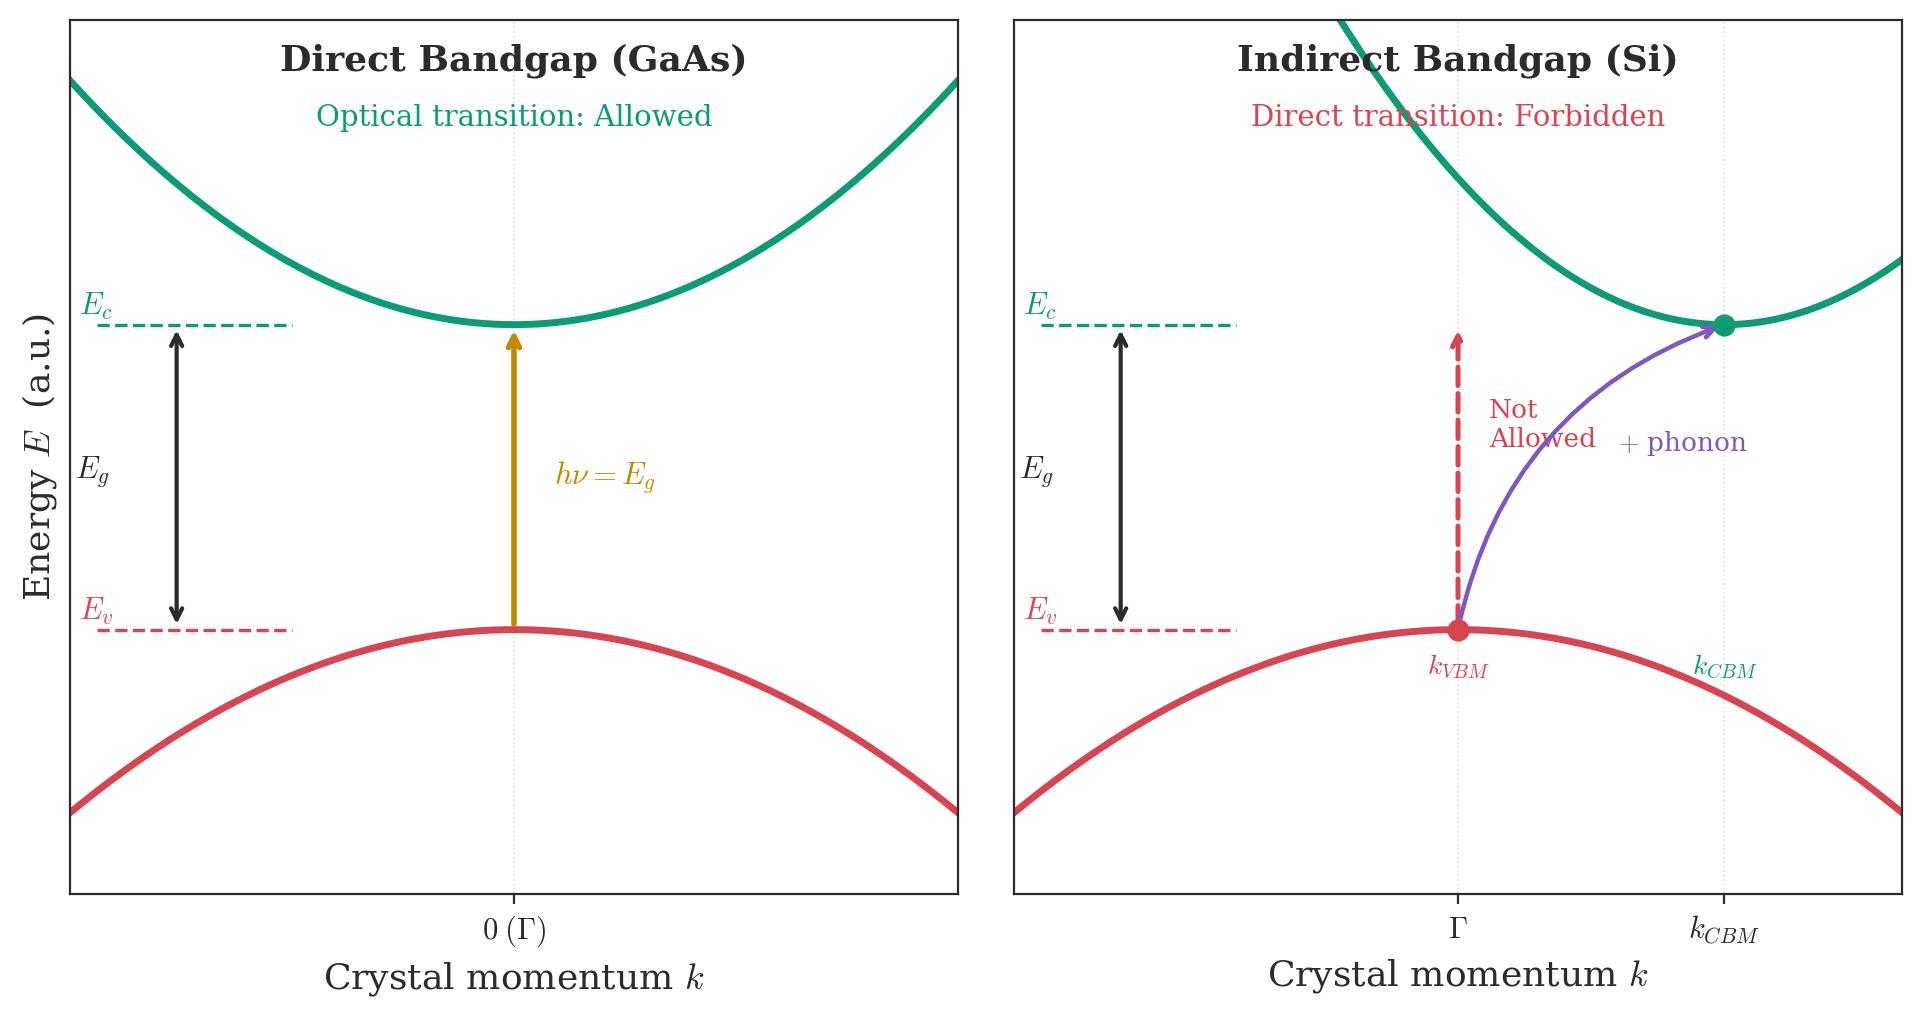
\includegraphics[width=0.6\textwidth]{Figures/Chapter 5/ek_band_structure.jpg}
    \caption{E–k Band Structure Diagram (Direct vs. Indirect)}
    \label{fig:ek_band_structure}
\end{figure}

\begin{itemize}
    \item \textbf{Direct bandgap semiconductor (e.g.\ GaAs):} The conduction band minimum and the valence band maximum occur at the \emph{same} k-point (the $\Gamma$ point, $k=0$). A vertical transition perfectly connects them. Optical emission is fully allowed, making GaAs the workhorse of laser diodes and LEDs.

    \item \textbf{Indirect bandgap semiconductor (e.g.\ Si):} The conduction band minimum sits at a different k-point from the valence band maximum. A vertical photon-only transition \emph{cannot} bridge the momentum gap. To complete the transition, a phonon (a quantised lattice vibration) must also be involved to supply the required crystal momentum. This three-particle process (electron + photon + phonon) is vastly less probable, making optical emission in Si extremely inefficient. This is why Si cannot be used to build practical LEDs or lasers.
\end{itemize}

The bottom line is fundamental: \textbf{only direct-bandgap semiconductors} make efficient light emitters.

% ------------------------------------------------------------------
\section{Density of States}
% ------------------------------------------------------------------

\subsection{The Concept: Counting Available Seats}

Before we can calculate how many electrons actually occupy the conduction band, we must first count how many \emph{quantum states} are available at each energy. This is the role of the \textbf{density of states} $g(E)$, which answers the question: how many states per unit volume exist in the energy range $[E,\, E+dE]$?

Think of it as a concert hall. $g(E)$ counts the number of seats at each energy level, and the Fermi-Dirac function $f(E)$ (which we will meet next) counts the fraction of those seats that are actually occupied. The total electron density is then simply seats $\times$ fraction occupied, integrated over all energies.

\subsection{Derivation in 3D}

To derive $g(E)$, we start with the known parabolic dispersion relation for a free-electron-like conduction band:
\begin{equation*}
    E = E_c + \frac{\hbar^2 k^2}{2 m^*_e}
\end{equation*}
We first count states in k-space. In a cubic crystal of side length $L$, periodic boundary conditions quantise the allowed $k$ values. The number of states in a spherical shell of radius $k$ and thickness $dk$ in 3D k-space is:
\begin{equation*}
    dN_k = 2 \cdot \frac{4\pi k^2\,dk}{(2\pi/L)^3} = \frac{V k^2\,dk}{\pi^2}
\end{equation*}
where the factor of 2 accounts for spin degeneracy (each k-state holds one spin-up and one spin-down electron), and $V = L^3$ is the volume. To convert from k to E, we differentiate the dispersion relation:
\begin{equation*}
    E - E_c = \frac{\hbar^2 k^2}{2m^*_e} \implies k = \sqrt{\frac{2m^*_e(E-E_c)}{\hbar^2}}
\end{equation*}
\begin{equation*}
    \frac{dE}{dk} = \frac{\hbar^2 k}{m^*_e} \implies dk = \frac{m^*_e}{\hbar^2 k}\,dE
\end{equation*}
Substituting $k = \sqrt{2m^*_e(E-E_c)}/\hbar$ and $dk = m^*_e\,dE/(\hbar^2 k)$ into the state-count expression $dN_k/V$ and cancelling the common factor of $\sqrt{2m^*_e(E-E_c)}/\hbar$ between numerator and denominator:
\begin{equation*}
    g_c(E) = \frac{1}{\pi^2}\cdot\frac{2m^*_e(E-E_c)}{\hbar^2}\cdot\frac{m^*_e}{\hbar^2}\cdot\frac{\hbar}{\sqrt{2m^*_e(E-E_c)}}
           = \frac{1}{\pi^2}\cdot\frac{m^*_e}{\hbar^3}\sqrt{2m^*_e(E-E_c)}
\end{equation*}
Writing $\hbar = h/(2\pi)$ and pulling the constants together:
\begin{equation*}
    g_c(E) = \frac{1}{\pi^2}\cdot\frac{m^*_e}{(h/2\pi)^3}\sqrt{2m^*_e(E-E_c)}
           = \frac{8\pi m^*_e}{h^3}\sqrt{2m^*_e(E-E_c)}
           = 4\pi\!\left(\frac{2m^*_e}{h^2}\right)^{\!3/2}\!\sqrt{E-E_c}
\end{equation*}
which gives us our density of states:
\begin{keyresult}
\begin{equation}
    g_c(E) = 4\pi\!\left(\frac{2m^*_e}{h^2}\right)^{\!3/2}\!\sqrt{E - E_c}, \qquad E \geq E_c
\end{equation}
\end{keyresult}
where $h = 2\pi\hbar$ is Planck's constant. By symmetry, the density of states for holes in the valence band has the same square-root form, with $m^*_e$ replaced by $m^*_h$ and $E_c$ replaced by $E_v$:
\begin{equation*}
    g_v(E) = 4\pi\!\left(\frac{2m^*_h}{h^2}\right)^{\!3/2}\!\sqrt{E_v - E}, \qquad E \leq E_v
\end{equation*}

The density of states grows as a square root above the band edge, which means there are very few states right at $E_c$, and the number of available seats increases as we move deeper into the band.

% ------------------------------------------------------------------
\section{The Fermi-Dirac Distribution}
% ------------------------------------------------------------------

Now that we have the seats, we need the occupancy rule. Quantum mechanics dictates that electrons — being fermions — obey the \textbf{Fermi-Dirac distribution}:
\begin{keyresult}
\begin{equation}
    f(E) = \frac{1}{1 + \exp\!\left(\dfrac{E - E_f}{k_B T}\right)}
\end{equation}
\end{keyresult}
where:
\begin{itemize}
    \item $f(E)$: the probability that a quantum state at energy $E$ is \emph{occupied} by an electron.
    \item $E_f$: the \textbf{Fermi energy} (or Fermi level) — the energy at which the occupation probability is exactly $1/2$.
    \item $k_B$: Boltzmann's constant.
    \item $T$: the absolute temperature in Kelvin.
\end{itemize}

The complementary probability that a state is \emph{empty} (occupied by a hole) is $[1 - f(E)]$. Notice that at $T = 0$ K, $f(E)$ becomes a perfect step function: every state below $E_f$ is filled, every state above is empty. At finite temperatures, this sharp step thermally smears over a window of width $\approx k_B T$ around $E_f$.

% ------------------------------------------------------------------
\section{Carrier Concentrations at Equilibrium}
% ------------------------------------------------------------------

\begin{figure}[H]
    \centering
    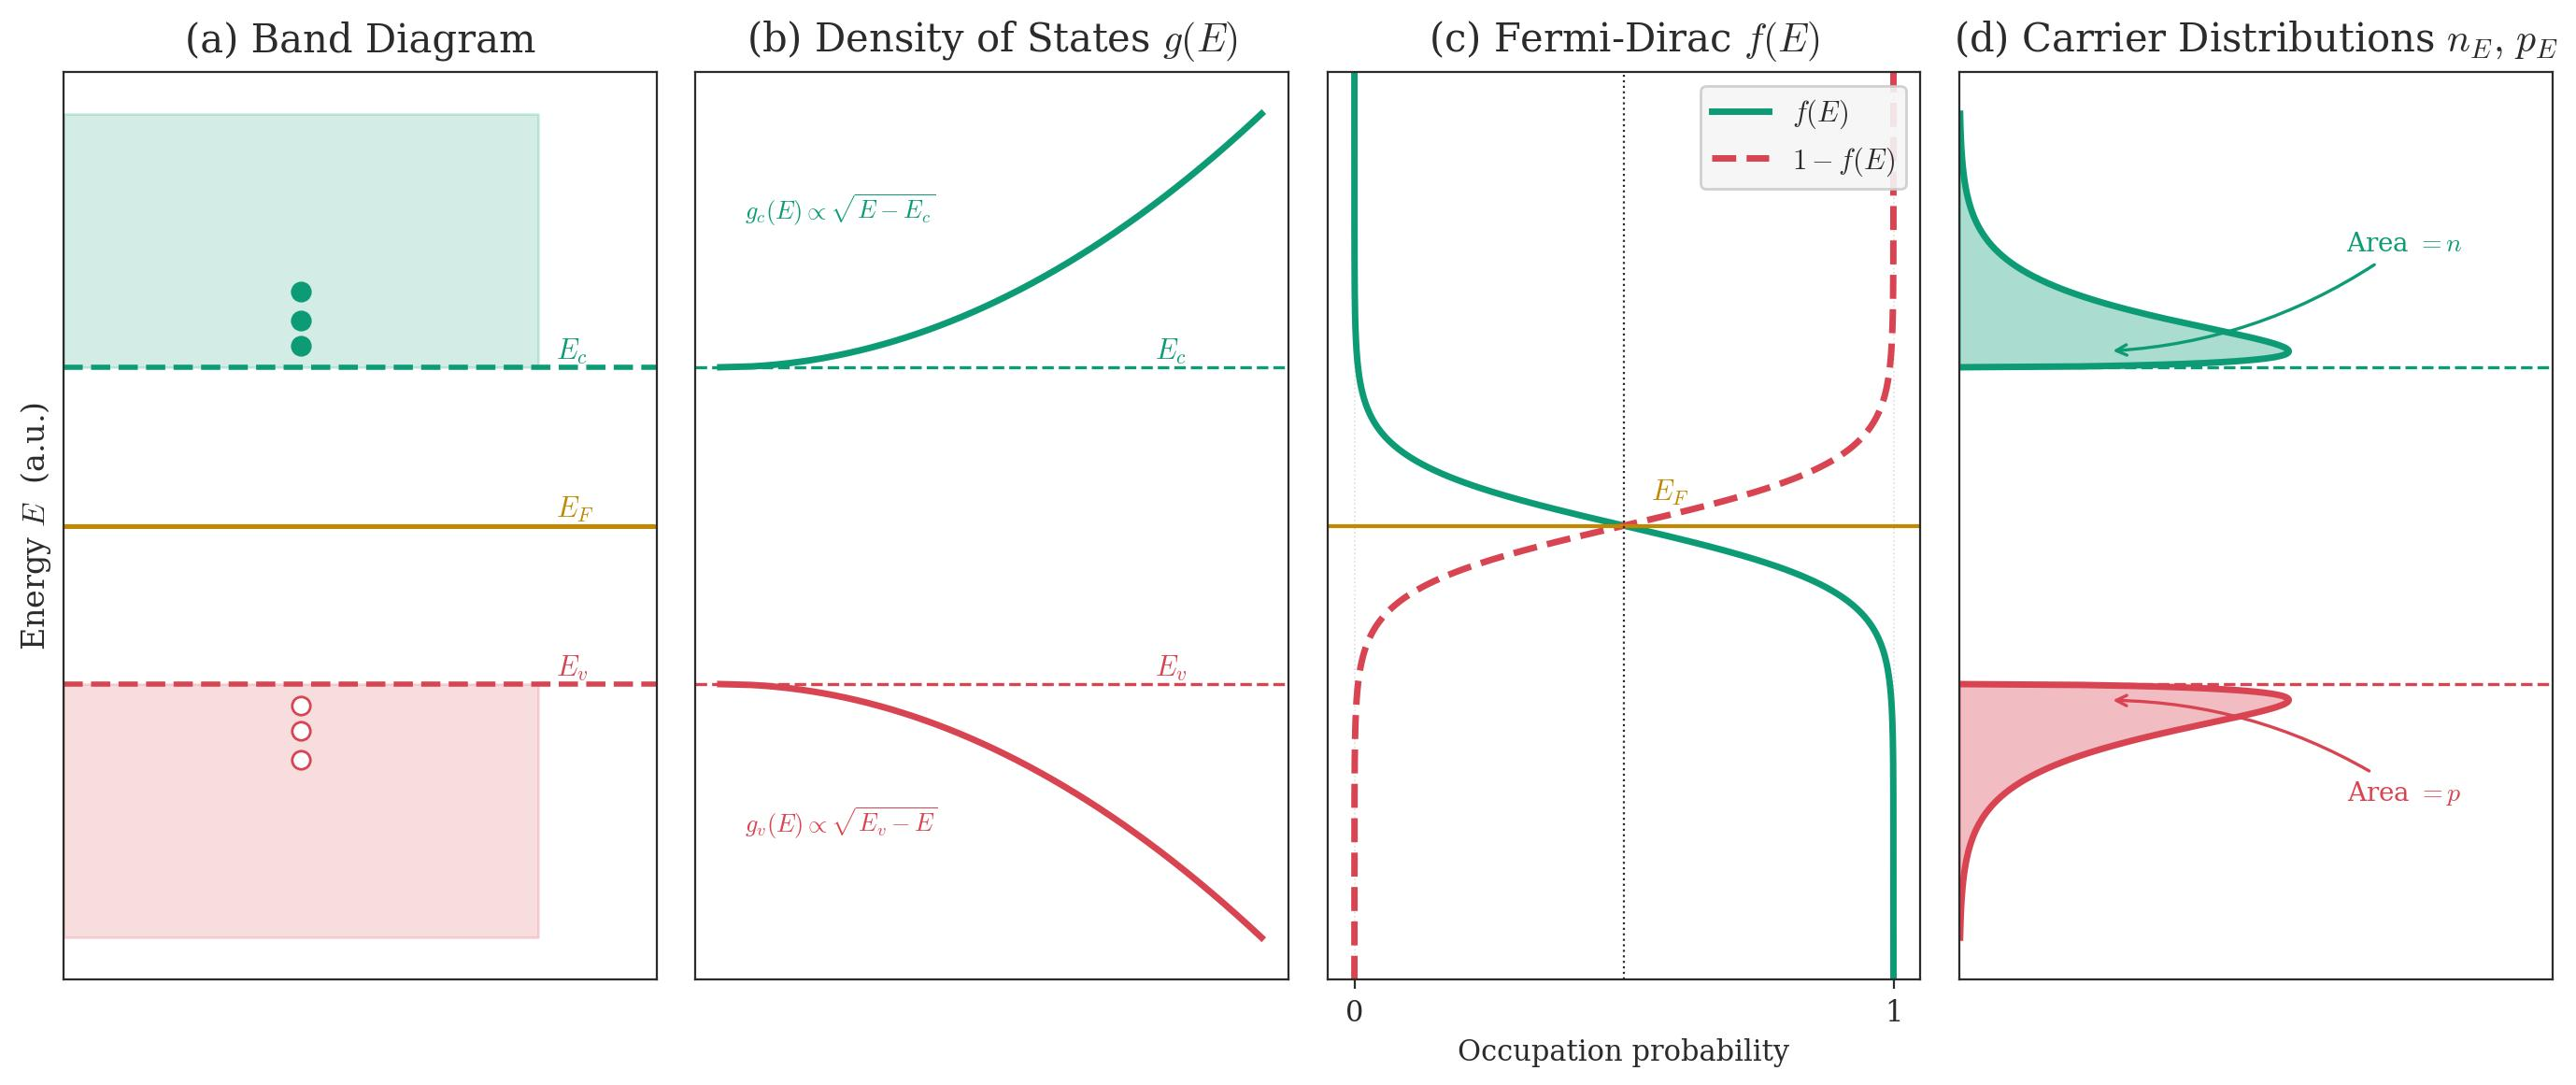
\includegraphics[width=0.6\textwidth]{Figures/Chapter 5/dos_carrier_distribution.jpg}
    \caption{Density of States and Carrier Distribution}
    \label{fig:dos_carrier_distribution}
\end{figure}

\subsection{The Integral Formula}

With both the density of states $g(E)$ and the occupation probability $f(E)$ in hand, the free electron density $n$ (electrons per unit volume in the conduction band) is just the integral of their product:
\begin{keyresult}
\begin{equation}
    n = \int_{E_c}^{\infty} g_c(E)\, f(E)\, dE
\end{equation}
\end{keyresult}

Substituting both expressions explicitly:
\begin{equation*}
    n = \int_{E_c}^{\infty} \frac{4\pi(2m^*_e/h^2)^{3/2}\sqrt{E - E_c}}{1 + \exp\!\left(\dfrac{E - E_f}{k_B T}\right)}\, dE
\end{equation*}

\subsection{The Maxwell-Boltzmann Approximation}

This integral has no closed form in general. However, in a non-degenerate semiconductor — one where the Fermi level sits well below the conduction band edge, specifically $E_c - E_f \gg k_B T$ — the exponential in the denominator is much greater than 1, and $f(E)$ simplifies to the \textbf{Maxwell-Boltzmann approximation}:
\begin{equation*}
    f(E) \approx \exp\!\left(-\frac{E - E_f}{k_B T}\right)
\end{equation*}

Substituting and factoring out the constant exponential involving $E_f$ and $E_c$:
\begin{equation*}
    n \approx 4\pi\!\left(\frac{2m^*_e}{h^2}\right)^{\!3/2}\exp\!\left(\frac{E_f - E_c}{k_B T}\right)\int_{E_c}^{\infty}\sqrt{E - E_c}\,\exp\!\left(-\frac{E - E_c}{k_B T}\right)dE
\end{equation*}

The remaining integral is a standard Gaussian integral. Substituting $u = (E-E_c)/k_B T$:
\begin{equation*}
    \int_0^\infty \sqrt{u}\,e^{-u}\,du = \frac{\sqrt{\pi}}{2}
\end{equation*}

Putting it all together and grouping the prefactor constants:
\begin{keyresult}
\begin{gather}
    n = N_c\,\exp\!\left(-\frac{E_c - E_f}{k_B T}\right) \\[1ex]
    N_c \equiv 2\!\left[\frac{2\pi m^*_e k_B T}{h^2}\right]^{\!3/2}
\end{gather}
\end{keyresult}
where $N_c$ is the \textbf{effective density of states in the conduction band} — a temperature-dependent constant that encapsulates the combined effect of the band curvature (via $m^*_e$) and the thermal energy available to the carriers. By an identical derivation for holes:
\begin{keyresult}
\begin{gather}
    p = N_v\,\exp\!\left(-\frac{E_f - E_v}{k_B T}\right) \\[1ex]
    N_v \equiv 2\!\left[\frac{2\pi m^*_h k_B T}{h^2}\right]^{\!3/2}
\end{gather}
\end{keyresult}

The physical picture is clean: the carrier density is simply the effective number of available states at the band edge $N_c$ (or $N_v$), thermally weighted by the Boltzmann factor that expresses how far the Fermi level is from that edge. The closer $E_f$ is to $E_c$, the more electrons are thermally excited into the conduction band.

\subsection{The Mass-Action Law}

Multiplying $n$ and $p$ together produces a particularly elegant result. All $E_f$ dependence cancels completely:
\begin{equation*}
    np = N_c N_v\,\exp\!\left(-\frac{E_c - E_v}{k_B T}\right) = N_c N_v\,\exp\!\left(-\frac{E_g}{k_B T}\right)
\end{equation*}

This product is a constant that depends only on the material (through $N_c$, $N_v$, and $E_g$) and the temperature — not on doping or the Fermi level position. We define the \textbf{intrinsic carrier concentration} $n_i$:
\begin{equation*}
    n_i^2 \equiv N_c N_v\,\exp\!\left(-\frac{E_g}{k_B T}\right)
\end{equation*}
giving us the \textbf{mass-action law}:
\begin{keyresult}
\begin{equation}
    np = n_i^2
\end{equation}
\end{keyresult}

This law is universal: it holds for intrinsic, n-doped, and p-doped semiconductors alike, as long as the material remains in thermal equilibrium. If we push more electrons into the CB by doping (increasing $n$), the hole density $p$ must decrease proportionally to keep the product constant. It is the semiconductor analogue of the chemical law of mass action.

% ------------------------------------------------------------------
\section{Non-Equilibrium Carriers and Quasi-Fermi Levels}
% ------------------------------------------------------------------

\subsection{Breaking Equilibrium}

Everything we have derived so far assumes \textbf{thermal equilibrium} — the semiconductor sits undisturbed, with a single, well-defined Fermi level $E_f$ governing both electrons and holes simultaneously. Lasers and LEDs operate in a fundamentally different regime.

When we forward-bias a PN junction or shine a strong pump beam onto a semiconductor, we inject excess carriers. The carrier populations are suddenly driven \emph{far away} from their equilibrium values. In this non-equilibrium state, there is no single Fermi level that simultaneously describes both electrons and holes.

Instead, we use a powerful but subtle trick: we assign \emph{two separate} quasi-Fermi levels, one for each carrier species. The electron quasi-Fermi level $E_{fn}$ describes the occupation of conduction band states:
\begin{keyresult}
\begin{equation}
    f_c(E) = \frac{1}{1 + \exp\!\left(\dfrac{E - E_{fn}}{k_B T}\right)}
\end{equation}
\end{keyresult}
and the hole quasi-Fermi level $E_{fp}$ describes the occupation of valence band states:
\begin{keyresult}
\begin{equation}
    f_v(E) = \frac{1}{1 + \exp\!\left(\dfrac{E - E_{fp}}{k_B T}\right)}
\end{equation}
\end{keyresult}

The modified carrier concentration expressions become:
\begin{equation*}
    n = N_c\,\exp\!\left(-\frac{E_c - E_{fn}}{k_B T}\right), \qquad p = N_v\,\exp\!\left(-\frac{E_{fp} - E_v}{k_B T}\right)
\end{equation*}

When excess electrons are injected into the CB, $E_{fn}$ shifts \emph{up} toward (or even into) the conduction band. When excess holes are injected into the VB, $E_{fp}$ shifts \emph{down} toward (or into) the valence band. The separation $E_{fn} - E_{fp}$ grows as injection increases. At equilibrium, $E_{fn} = E_{fp} = E_f$.

\begin{figure}[H]
    \centering
    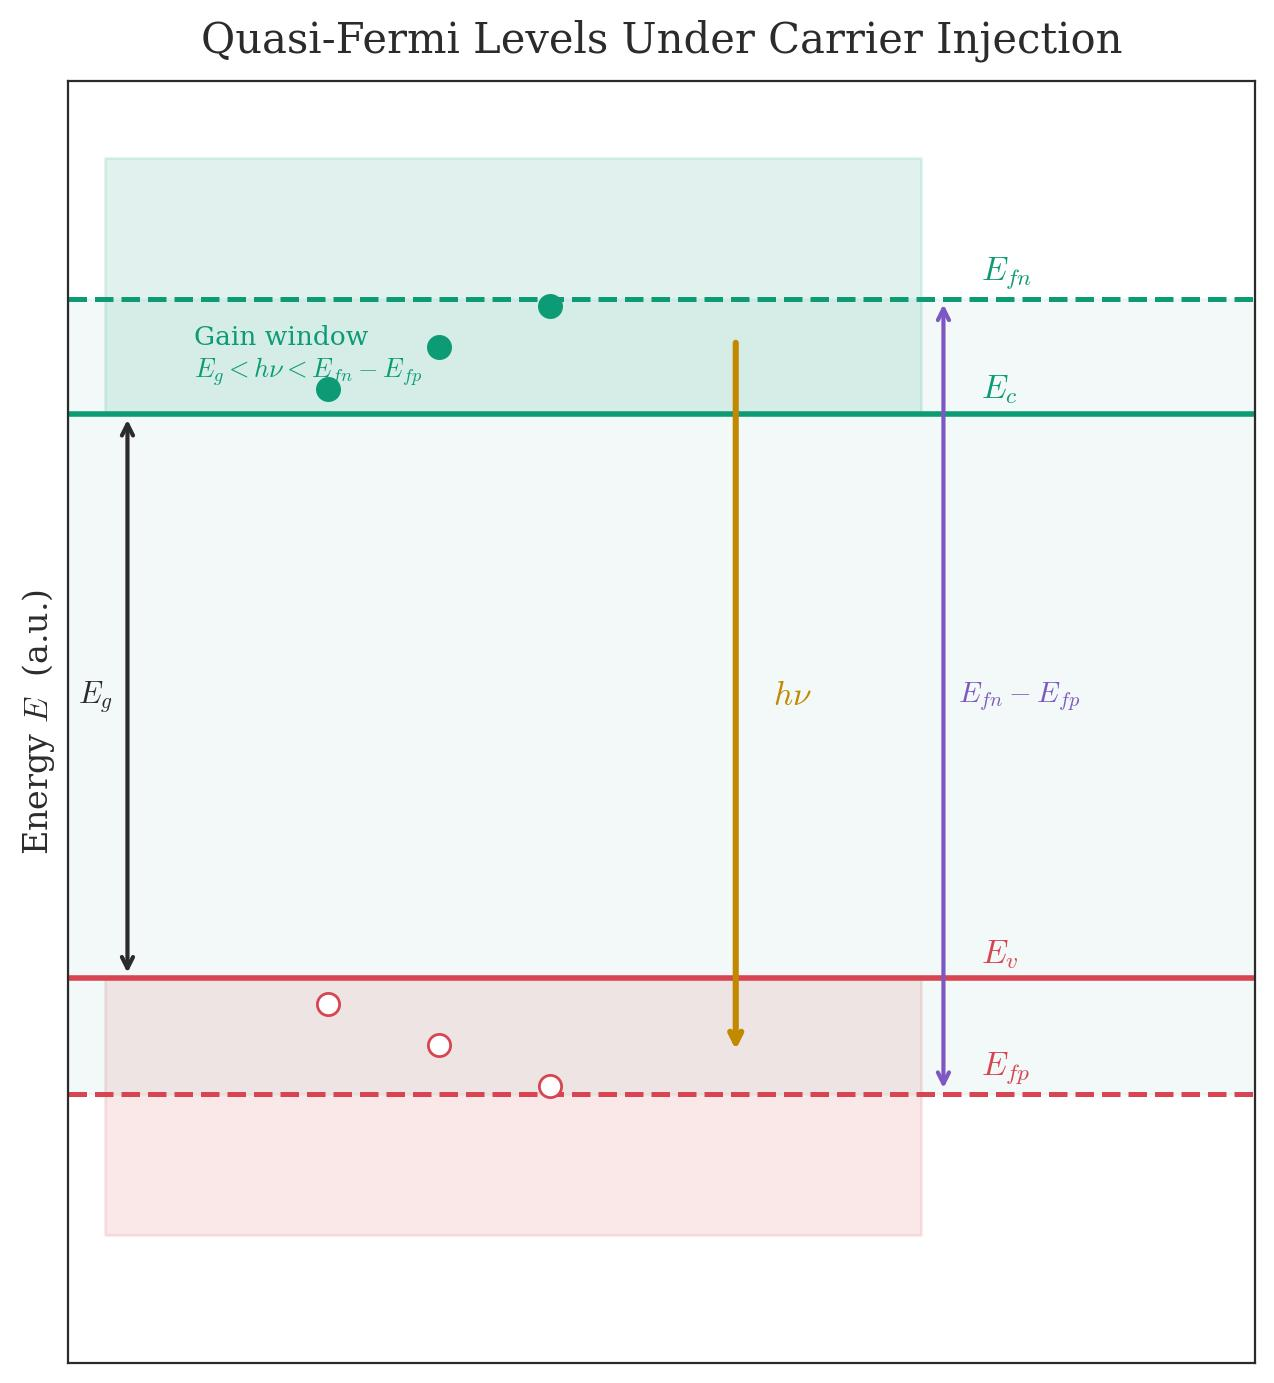
\includegraphics[width=0.6\textwidth]{Figures/Chapter 5/quasi_fermi_levels.jpg}
    \caption{Quasi-Fermi Levels Under Injection}
    \label{fig:quasi_fermi_levels}
\end{figure}

\subsection{The Physical Justification}

Why does this two-quasi-Fermi-level picture make sense? Carriers reach thermal equilibrium within their own band extremely fast — via intraband carrier-carrier and carrier-phonon scattering, on a timescale of roughly $10^{-13}$ s (100 fs). This rapid intraband thermalisation means electrons in the CB quickly distribute themselves among CB states according to a Fermi-Dirac distribution characterised by their own quasi-Fermi level $E_{fn}$. Holes in the VB do the same with $E_{fp}$. The \emph{interband} recombination (electron falling from CB to VB) is vastly slower — nanoseconds — so the two populations do not equilibrate with each other on the timescales of interest. Two separate quasi-Fermi levels are therefore an excellent approximation.

% ------------------------------------------------------------------
\section{The Gain Condition and Population Inversion}
% ------------------------------------------------------------------

\subsection{Population Inversion in a Two-Level Picture}

To achieve optical gain — where stimulated emission exceeds absorption — we need population inversion. For a photon of energy $h\nu$ interacting with an electron at energy $E_2$ in the CB and a hole at energy $E_1$ in the VB, stimulated emission dominates absorption when the probability of finding the upper state occupied \emph{and} the lower state empty exceeds the reverse:
\begin{equation*}
    f_c(E_2)\bigl[1 - f_v(E_1)\bigr] > f_v(E_1)\bigl[1 - f_c(E_2)\bigr]
\end{equation*}
Expanding and cancelling common terms, this simplifies to:
\begin{equation*}
    f_c(E_2) > f_v(E_1)
\end{equation*}

\subsection{Why a Single Material Cannot Achieve This}

Now, in a single material at equilibrium with one Fermi level $E_f$, we would need:
\begin{equation*}
    \frac{1}{1+\exp\!\left(\dfrac{E_2 - E_f}{k_B T}\right)} > \frac{1}{1+\exp\!\left(\dfrac{E_1 - E_f}{k_B T}\right)}
\end{equation*}
Since $f(E)$ is a strictly decreasing function of $E$, this requires $E_2 < E_1$. But $E_2$ is in the conduction band and $E_1$ is in the valence band, so $E_2 > E_1$ always. \textbf{Population inversion is impossible in a single material at equilibrium.} This is a fundamental result.

\subsection{The PN Junction Solution and the Bernard-Duraffourg Condition}

The resolution is to use a forward-biased PN junction, which provides two separate quasi-Fermi levels. The gain condition becomes:
\begin{equation*}
    \frac{1}{1+\exp\!\left(\dfrac{E_2 - E_{fn}}{k_B T}\right)} > \frac{1}{1+\exp\!\left(\dfrac{E_1 - E_{fp}}{k_B T}\right)}
\end{equation*}
Following the same algebraic steps — the Fermi-Dirac inequality reduces to requiring $E_2 - E_{fn} < E_1 - E_{fp}$, which rearranges to:
\begin{equation*}
    E_{fn} - E_{fp} > E_2 - E_1
\end{equation*}
Since $E_2 - E_1 = h\nu$ (energy conservation of the photon), and since the photon energy must be at least $E_g$ to span the bandgap, we arrive at the celebrated \textbf{Bernard-Duraffourg condition}:
\begin{keyresult}
\begin{equation}
    E_{fn} - E_{fp} > h\nu > E_g
\end{equation}
\end{keyresult}

This is the central result of semiconductor laser physics. Let's unpack what it demands physically:

\begin{itemize}
    \item $h\nu > E_g$: The photon must have enough energy to bridge the bandgap and stimulate a real interband transition. Photons with energy below $E_g$ are transparent to the material.
    \item $E_{fn} - E_{fp} > h\nu$: The quasi-Fermi level separation must exceed the photon energy. This is the inversion condition — it guarantees that the conduction band state $E_2$ is more likely to be occupied than the valence band state $E_1$.
    \item Together: The quasi-Fermi level separation must be larger than the bandgap, $E_{fn} - E_{fp} > E_g$, which in practice requires heavy carrier injection achieved via strong forward bias.
\end{itemize}

Ultimately, what this tells us is that a semiconductor laser operates in a window: photon energies between $E_g$ and $(E_{fn} - E_{fp})$ will experience net gain. Outside this window, either the photon is too weak to cross the gap, or inversion does not exist for that transition. The width of this gain window grows as we push more current (more injection) into the device, spreading the quasi-Fermi levels further apart.

\begin{figure}[H]
    \centering
    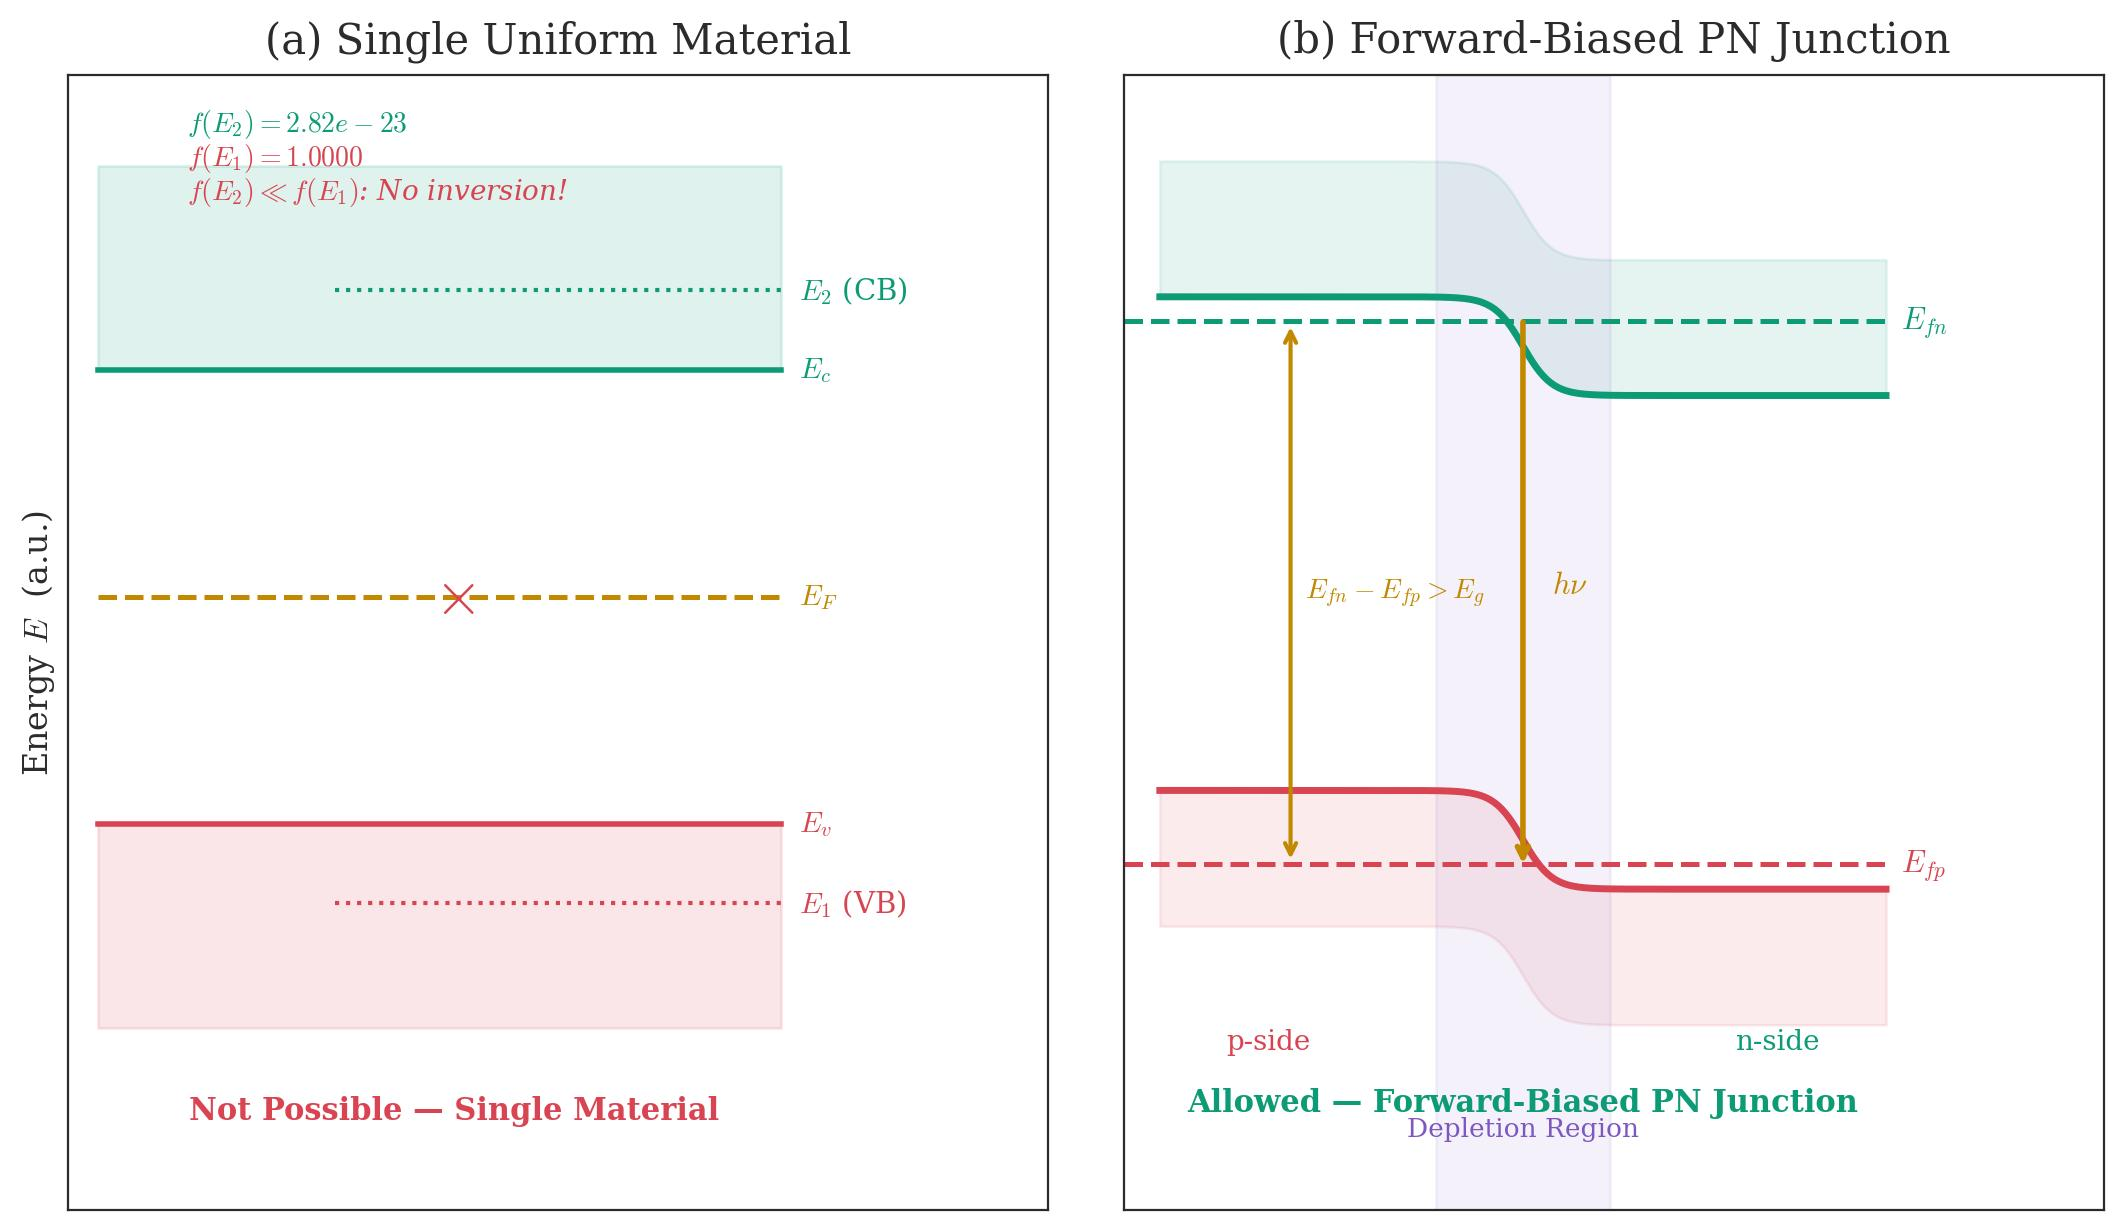
\includegraphics[width=0.6\textwidth]{Figures/Chapter 5/population_inversion_condition.jpg}
    \caption{Population Inversion Condition — Single Material vs. PN Junction}
    \label{fig:population_inversion_condition}
\end{figure}

% ------------------------------------------------------------------
\section{The Homojunction Diode}
% ------------------------------------------------------------------

\subsection{Three Operating Regimes}

The simplest structure that can achieve population inversion is the \textbf{homojunction} — a PN junction made of a single semiconductor material (same composition, different doping on each side). Understanding its three bias regimes builds the intuition needed for the more advanced double-heterostructure lasers we will study later.

\textbf{(a) Equilibrium (zero bias):} At zero bias, the built-in electric field across the depletion region — arising from the diffusion of carriers and the resulting fixed-charge layer — creates a built-in potential $eV_0$. This potential bends the conduction and valence band edges, establishing a built-in barrier that exactly prevents net current flow. A single Fermi level $E_f$ runs flat and continuous across the entire device (n-side, depletion region, p-side). Electrons are confined to the n-side, holes to the p-side.

\textbf{(b) Forward bias ($V > 0$):} Applying a forward voltage $V$ lowers the built-in barrier to $e(V_0 - V)$. Electrons from the n-side are injected across the junction into the p-side, and holes from the p-side are injected into the n-side. Within the depletion/recombination region, the two quasi-Fermi levels $E_{fn}$ and $E_{fp}$ are now separated by exactly $eV$:
\begin{equation*}
    E_{fn} - E_{fp} = eV
\end{equation*}
This separation grows linearly with the applied voltage. At moderate forward bias, $eV < E_g$, and stimulated emission at the bandgap is not yet possible.

\textbf{(c) High forward bias (transparency and gain):} As the voltage increases further toward $eV \approx E_g$, the quasi-Fermi level separation approaches the bandgap. Once $eV > E_g$, the Bernard-Duraffourg condition $E_{fn} - E_{fp} > h\nu > E_g$ is satisfied within the active recombination region, and net optical gain is achieved. The junction becomes a source of stimulated emission.

Both quasi-Fermi levels coexist \emph{simultaneously} inside the depletion region — this is the crucial point. The n-side has $E_{fn}$ close to its conduction band; the p-side has $E_{fp}$ close to its valence band. In the depletion region, both coexist, providing the separated electron and hole populations needed for gain.

\begin{figure}[H]
    \centering
    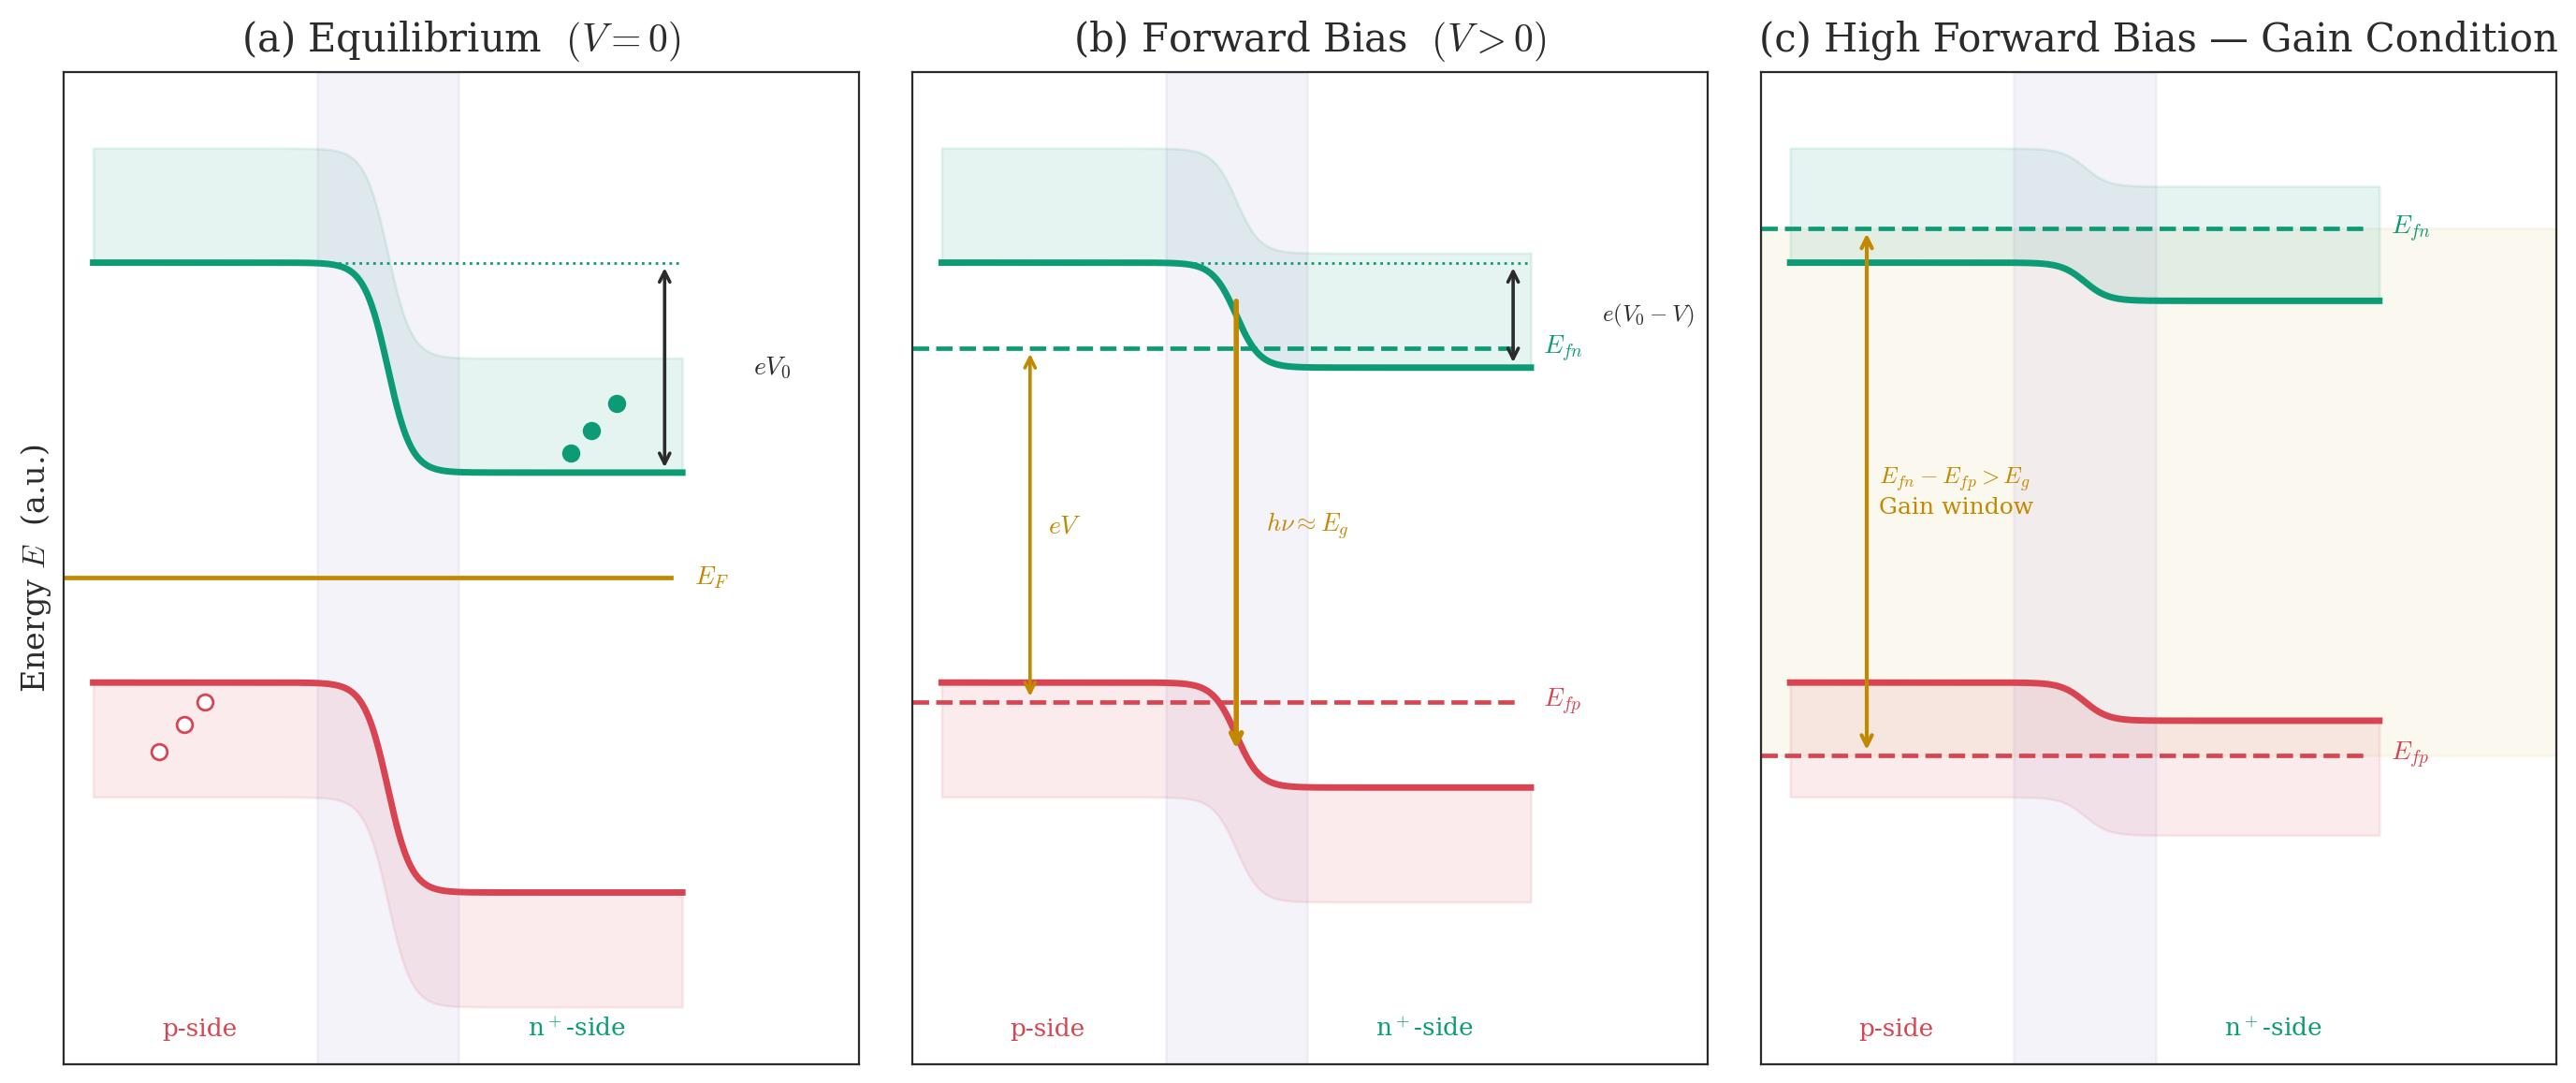
\includegraphics[width=0.7\textwidth]{Figures/Chapter 5/homojunction_bias_states.jpg}
    \caption{Homojunction Band Diagram — Three Bias States}
    \label{fig:homojunction_bias_states}
\end{figure}

\begin{keyinsight}[The Limitation of the Homojunction]
The homojunction has a fundamental practical limitation: the injected carriers are not confined. Electrons injected into the p-side simply diffuse away over a diffusion length $L_D \sim 1$--$10\,\mu$m before recombining. This means the gain region is large, and the threshold current density required to achieve inversion is dauntingly high (of order $10^4$--$10^5$ A/cm$^2$). This limitation motivates the double-heterostructure laser design, where two abrupt bandgap changes create a potential well that physically traps both electrons and holes within a thin active layer of a few hundred nanometres, dramatically reducing the threshold current. That structure will be the subject of the next chapter.
\end{keyinsight}
